% \documentclass{article}

% %----------------------------------------------------------------------------------------
% %	PACKAGES AND THEMES
% %----------------------------------------------------------------------------------------
% \usepackage[utf8]{inputenc} % Allow input to be UTF-8
% \usepackage[T1]{fontenc}    % Use 8-bit T1 fonts
% \usepackage{url}            % Simple URL typesetting
% \usepackage{booktabs}       % Professional-quality tables
% \usepackage{amsfonts}       % Blackboard bold symbols
% \usepackage{nicefrac}       % Compact symbols for 1/2, etc.
% \usepackage{microtype}      % Microtypography
% \usepackage{xcolor}         % Colors
% \usepackage{amsmath}        % Math packages
% \usepackage{amssymb}
% \usepackage{graphicx}       % For images
% \usepackage{natbib}         % For Author-Year citations (ICLR style)
% \usepackage{geometry}       % Layout management

% % Simulate ICLR/NeurIPS Preprint Layout
% \geometry{
%     a4paper,
%     total={138mm,210mm}, % Approx ICLR text width
%     left=36mm,
%     top=36mm,
% }

% % Title Formatting
% \usepackage{titlesec}
% \titleformat{\section}{\large\bfseries}{\thesection}{1em}{}
% \titleformat{\subsection}{\normalsize\bfseries}{\thesubsection}{1em}{}

% % Hyperlinks setup
% \usepackage{hyperref}
% \hypersetup{
%     colorlinks=true,
%     linkcolor=red,
%     filecolor=magenta,      
%     urlcolor=blue,
%     citecolor=blue,
% }

% %----------------------------------------------------------------------------------------
% %	TITLE AND AUTHORS
% %----------------------------------------------------------------------------------------
% \title{\textbf{HIEU: Hypernetwork-Integrated Expert Unit for \\ Robust and Interpretable Multi-Asset Forecasting}}

% \author{
%   \textbf{Hieu Duc} \\
%   Hephaestus Tech AI Research Lab \\
%   \texttt{hieu.pham@hephaestus-tech.org}
% }
% \date{} % No date for conference submissions

% \begin{document}

% \maketitle

% %----------------------------------------------------------------------------------------
% %	ABSTRACT
% %----------------------------------------------------------------------------------------
% \begin{abstract}
% As deep learning models become increasingly embedded in critical decision-making processes—from medical diagnostics to high-frequency financial trading—the demand for explainability has grown alongside the need for accuracy. Current state-of-the-art forecasting models often excel at capturing long-range dependencies but remain opaque "black boxes." In this work, we propose the \textbf{Hypernetwork-Integrated Expert Unit (HIEU)}, a novel architecture that bridges the gap between robust linear modeling and deep adaptability. HIEU explicitly decouples the context of data from the mechanism of prediction using a Hypernetwork conditioned on a transparent "Multi-View Context": Market Regime, Graph Structure, and Frequency Patterns. Our approach offers a "Glass Box" paradigm, allowing users to inspect detected regimes and cross-asset correlations, providing the trust essential for deployment in volatile environments.
% \end{abstract}

% %----------------------------------------------------------------------------------------
% %	1. INTRODUCTION
% %----------------------------------------------------------------------------------------

%%%% ijcai26.tex

\typeout{IJCAI--ECAI 26 Instructions for Authors}

% These are the instructions for authors for IJCAI--ECAI 26.

\documentclass{article}
\pdfpagewidth=8.5in
\pdfpageheight=11in

% The file ijcai26.sty is a copy from ijcai22.sty
% The file ijcai22.sty is NOT the same as previous years'
\usepackage{ijcai26}

% Use the postscript times font!
\usepackage{times}
\usepackage{soul}
\usepackage{url}
\usepackage[hidelinks]{hyperref}
\usepackage[utf8]{inputenc}
\usepackage[small]{caption}
\usepackage{graphicx}
\usepackage{amsmath}
\usepackage{amsthm}
\usepackage{graphicx}
\usepackage{amsfonts} 
\usepackage{subcaption}
\usepackage{natbib}
\usepackage{booktabs}

\usepackage{siunitx}

\usepackage{algorithm}
\usepackage{multirow} 

\usepackage{adjustbox}

\usepackage{algorithmic}
\usepackage[switch]{lineno}

% Comment out this line in the camera-ready submission
\linenumbers

\urlstyle{same}

% the following package is optional:
%\usepackage{latexsym}

% See https://www.overleaf.com/learn/latex/theorems_and_proofs
% for a nice explanation of how to define new theorems, but keep
% in mind that the amsthm package is already included in this
% template and that you must *not* alter the styling.
\newtheorem{example}{Example}
\newtheorem{theorem}{Theorem}

% Following comment is from ijcai97-submit.tex:
% The preparation of these files was supported by Schlumberger Palo Alto
% Research, AT\&T Bell Laboratories, and Morgan Kaufmann Publishers.
% Shirley Jowell, of Morgan Kaufmann Publishers, and Peter F.
% Patel-Schneider, of AT\&T Bell Laboratories collaborated on their
% preparation.

% These instructions can be modified and used in other conferences as long
% as credit to the authors and supporting agencies is retained, this notice
% is not changed, and further modification or reuse is not restricted.
% Neither Shirley Jowell nor Peter F. Patel-Schneider can be listed as
% contacts for providing assistance without their prior permission.

% To use for other conferences, change references to files and the
% conference appropriate and use other authors, contacts, publishers, and
% organizations.
% Also change the deadline and address for returning papers and the length and
% page charge instructions.
% Put where the files are available in the appropriate places.


% PDF Info Is REQUIRED.

% Please leave this \pdfinfo block untouched both for the submission and
% Camera Ready Copy. Do not include Title and Author information in the pdfinfo section
\pdfinfo{
/TemplateVersion (IJCAI.2026.0)
}

\title{HIEU: Regime-Aware Hypernetwork Experts for Explainable \\ Multi-Asset Cryptocurrency Forecasting}

% Single author syntax
\author{
    Anonymous
    \affiliations
    Anonymous
    \emails
    anonymous@anonymous.com
}

% Multiple author syntax (remove the single-author syntax above and the \iffalse ... \fi here)
\iffalse
\author{
First Author$^1$
\and
Second Author$^2$\and
Third Author$^{2,3}$\And
Fourth Author$^4$\\
\affiliations
$^1$First Affiliation\\
$^2$Second Affiliation\\
$^3$Third Affiliation\\
$^4$Fourth Affiliation\\
\emails
\{first, second\}@example.com,
third@other.example.com,
fourth@example.com
}
\fi

\begin{document}

\maketitle

\begin{abstract} 
Despite promising results from state-of-the-art general time-series predictive models, their direct applications in cryptofinance are undermined by the lack of domain-specific consideration of multi-asset interactions, cryptocurrency regimes, and model explainability for reliable decision-making. Therefore, we propose HIEU, a novel hypernetwork of experts that dynamically generates context-conditioned low-rank weight adaptations based on a rich multi-view context vector fusing regime, time-evolving cross-asset graph relationships, and multi-scale frequency patterns. Our approach enables sample-specific, regime-aware forecasting that captures inter-asset dependencies and temporal shifts while remaining parameter-efficient. Notably, HIEU offers intrinsic glass-box explainability through interpretable regime probabilities, graph heatmaps, frequency gating weights, and optional post-hoc analysis on the context vector, ultimately delivering probabilistic quantile predictions tailored for risk-sensitive multi-asset cryptocurrency trading. Having outperformed prominent time-series Transformers and deep learning variants in validation metrics alongside architectural design, HIEU advances the engineering of adaptive, explainable forecasting models for real-world volatile financial trading platforms.
\end{abstract}

\section{Introduction}
Financial time series, particularly cryptocurrencies, present unique challenges due to their chaotic, non-stationary nature driven by numerous interdependent yet unpredictable factors. This distinguishes crypto time series from other domains. Moreover, investors typically hold diversified portfolios across different market regimes, further increasing the complexity and uncertainty of influential factors.

Therefore, SoTA time-series models would instantly fail in financial trading environments due to the lack of consideration for the aforementioned factors. This has motivated the work of (1) utilizing deep learning models for multivariate forecasting, relying on their neural ability to learn underlying patterns of the crypto time series across engineered features and ensemble methods, or (2) studying the obvious “black box” nature of deep neural models to understand influential variables behind the output decision. In particular, Transformer-based models \citep{patchtst, autoformer, informer} excel at capturing long-range dependencies but remain largely inexplainable due to inherent attention-mechanism entanglement, where learned attention weights do not correspond to interpretable temporal or feature-wise importance. Conversely, hybrid linear models \citep{boo} offer transparency against distribution shifts but lack the capacity to capture cross-asset relationships in non-stationary markets. Nevertheless, strong opacity is dangerous in high-stakes environments, where sequences of decisions are made per second. Hence, users should be able to acknowledge whether a correlation shift or regime switch is behind the predicted outcome. Otherwise, the action of trading is contemplated as a evenly probabilistic decision, which does not benefit the study of digital finance. Concerning explainability, recent research has attempted to clear the models’ black box via post-hoc explanations: perturbation-based approaches \citep{pertubation} assess prediction sensitivity by modifying or removing parts of the input; attribution-based approaches \citep{attribution} assign importance scores to input features based on their contribution to the output. However, these approaches rely on masking or blurring individual time steps, which can break meaningful long-term temporal patterns, leading to poor explanations.


We pose the research question: \textit{How to build SoTA explainable, adaptive units that swiftly respond to cryptocurrency regimes and inter-asset relationships?}. As a result, this study proposes HIEU (\textbf{H}ypernetwork-\textbf{I}ntegrated \textbf{E}xpert \textbf{U}nit), a novel architecture that bridges the gap between interpretable linear modeling and regime-aware capability. Instead of relying on static weights, HIEU utilizes a hypernetwork to rapidly generate time-step-specific forecasting weights conditioned on a transparent multi-view market context that includes the current market regime (e.g., Bull, Bear, Volatile), the learned graph structure capturing cross-asset correlations, and multi-scale frequency patterns extracted via finite impulse response-based temporal decomposition. By grounding the prediction on these explicit factors, HIEU offers  glass-box approach as users can inspect which regime the model detected and how assets are currently correlated, providing the trust essential for deployment in chaotic environments.





%----------------------------------------------------------------------------------------
%	2. BACKGROUND
%----------------------------------------------------------------------------------------
\newpage
\section{Literature Review}
\subsection{Related Work}
\label{relatedwork}

\noindent\textbf{a) Single architectures.} 
Initially, studies on financial time series forecasting progressed from conventional statistical techniques to more sophisticated machine learning (ML) and deep learning (DL) methods. Regression-based approaches, such as linear regression, often serve as fundamental benchmarks. Particularly, \citet{a2} demonstrated that Autoregressive Integrated Moving Average (ARIMA) models outperformed basic linear regression, although they tended to produce excessively linear projections. Similarly, \citet{a1} tailored an ARIMA model to 9-month Bitcoin data, identifying ARIMA(0,2,1) as the optimal configuration, which achieved a Mean Absolute Percentage Error (MAPE) of 3.17\%. ARIMA tends to deliver acceptable results for short-term predictions in stable conditions but exhibits substantial errors during extended periods of high market turbulence \citep{a3}, highlighting its dependence on appropriate window sizes and parameter tuning. Traditional parametric models, including (Seasonal)ARIMA, linear regression (LR), and GARCH, depend on explicit functional forms that relate historical values or external variables to future outcomes, offering interpretability \citep{extra}. 

Nevertheless, the linear nature of classical models restricts their effectiveness on highly volatile datasets, driving interest toward ML/DL techniques that automatically identify intricate patterns in time series data, albeit at the cost of lower interpretability. When applied to Bitcoin and Ethereum price records from 2013 to 2019, Long Short-Term Memory (LSTM) networks yielded superior performance over basic Recurrent Neural Networks (RNNs), recording lower Root Mean Squared Error (RMSE) values (0.061 for BTC and 0.036 for ETH) and MAPE (5.66\% for BTC and 4.58\% for ETH) \citep{a6}. On the same crypto pairs, Gated Recurrent Unit (GRU) models surpassed LSTM, delivering even smaller MAPE (0.38\% for BTC and 0.45\% for ETH) and higher R² scores (0.9988 for BTC and 0.9983 for ETH) \citep{a7}. Evaluations on S\&P500 constituents, using Open-High-Low-Close-Volume (OHLCV) inputs, showed that LSTM consistently outperformed traditional statistical methods (e.g., ARIMA, GARCH) and ML baselines in terms of Mean Squared Error (MSE) and RMSE, thanks to its gating mechanisms that enable selective memory retention and information flow over time \citep{anh1, anh2}. 

Latest Transformer-based architectures \citep{informer, autoformer, patchtst} have achieved SoTA results in multivariate time series forecasting due to their progressive series decomposition with auto-correlation mechanism, probabilistic sparse self-attention with self-attention distillation, and subseries-level patching combined with channel-independent processing. However, Autoformer \citep{autoformer}, Informer \citep{informer}, and FEDFormer \citep{fedformer} were surpassed by a one-layer linear model in long-term time series forecasting on general datasets (e.g., ETTh1, Electricity, Traffic) \citep{boo}. In addition, Transformer-based adoption for applied cryptocurrency price forecasting is still poorly explored.


\noindent\textbf{b) Hybrid architectures.}
Hybrid frameworks extend beyond individual models by integrating multiple components or complementary techniques to enhance input representation and contextual understanding. A notable example is the CLAM architecture \citep{clam}, which stacks multiple CNN layers for spatial feature learning, followed by LSTM layers to model sequential patterns, and concludes with an attention layer at the prediction stage to emphasize important information. This combination resulted in an approximately 80\% reduction in MAE and RMSE, along with 75\% accuracy in predicting one-week-ahead trends for S\&P500 stocks. Applying these principles, \citet{a8} reported that a CNN-LSTM hybrid significantly outperformed standalone CNN or LSTM variants, achieving half the MAE and MSE when forecasting recent Bitcoin closing prices. Comparable ensemble-style hybrids have also been explored \citep{nisha, hybrid1, a9}, consistently yielding 30--50\% reductions in MSE, MAE, and MAPE across various cryptocurrency pairs (e.g., BTC, XRP, DOGE) relative to single-model baselines.

Beyond pure ensembling, certain designs exploit cross-series correlations or external signals aligned with time. For example, \citet{hybrid5} incorporated trend predictions generated by a Large Language Model (LLM) in the form of one-hot encoded directions and associated probabilities derived from prompts that combine financial news, stock characteristics, and past closing prices. These LLM-derived features were fed into a Transformer architecture, which delivered better next-day stock price forecasts than LSTM, CNN-LSTM, Random Forest, XGBoost, and standard Transformer models.  Likewise, \citet{a10} fused CNN-LSTM processing of Bitcoin price data with sentiment features extracted from Twitter and Reddit posts, resulting in 7--9\% higher predictive accuracy compared to isolated CNN or LSTM implementations. The inclusion of sentiment information, combined with attention weighting, proved especially valuable for improving forecasts. Other similar efforts include FinBERT-LSTM \citep{a11}, which integrated financial sentiment from news hierarchies with LSTM modeling of lagged prices for NASDAQ-100 predictions, and ARDL-MIDAS \citep{a12}, which combined mixed-frequency regression with Transformer attention, using daily entropy-informed cryptocurrency sentiment as the target variable and hourly price/technical factors as regressors to support intra-day end-of-day sentiment forecasting.


%----------------------------------------------------------------------------------------
%	3. METHOD
%----------------------------------------------------------------------------------------
% \section{Methodolgy}
% \subsection{Problem Formulation}
% We consider the problem of multi-asset time series forecasting. Let $\mathbf{X} \in \R^{B \times L \times N}$ denote the input tensor, where $B$ is the batch size, $L$ is the look-back window length, and $N$ is the number of assets. The objective is to predict the future values $\mathbf{Y} \in \R^{B \times S \times N}$ for a forecast horizon $S$. Additionally, to quantify uncertainty, the model must estimate a set of $Q$ quantiles $\mathbf{Q}_{pred} \in \R^{B \times S \times Q \times N}$.

\subsection{Research Problem}
Despite architectural novelty (Section \ref{relatedwork}), these predictive frameworks remain fundamentally limited when applied to cryptocurrency time series due to following fundamental bottlenecks: Transformer-based variants with the multi-head self-attention mechanism \citep{attention} are largely opaque due to their non-linear structure, stacked layers, residual connections, activation functions, and entangled intermediate representations \citep{b1}. These construct black-box characters that hinder financial interpretability. 

Recent research does advance in deep neural model explainability via pertubation or attribution-based methods \citep{pertubation, attribution, b3}. However, these post-hoc explanation techniques predominantly capture correlative rather than causal relationships and remain vulnerable to adversarial perturbations or out-of-distribution shifts commonly encountered in cryptocurrency markets \citep{shapley, gradient}. Consequently, they offer limited actionable insight for risk-sensitive financial applications because such frameworks cannot determine whether a predicted price downturn stems from a sudden shift in cross-asset correlations, an underlying regime transition, or clustering of shocks.


Alternatively, static linear forecasters \citep{boo}, while outperforming Transformer variants and offering greater efficacy by relying on fixed weight matrices $\mathbf{W} \in \mathbb{R}^{S \times L}$ to produce predictions in the form $\hat{\mathbf{Y}} = \mathbf{W}\mathbf{X} + \mathbf{b}$ after trend decomposition, assume time-invariant mappings. Therefore, they fail to adapt to the markedly dynamic, time-varying cross-asset covariances, lead-lag structures, and evolving dependency patterns that characterize cryptocurrency markets \citep{b4}. When linear models are trained via empirical risk minimization on historical data, their performance often degrades once the underlying joint distribution undergoes a concept drift \citep{b5}.

Compounding these issues is the almost complete absence of straightforward regime awareness. Cryptocurrency markets frequently transition between distinct latent states (e.g., bull, bear, sideways) and each is characterized by markedly different conditional densities and autocorrelation structures \citep{b7}. Investors’ portfolio are also diversified, holding cryptocurrencies from distinctive indexes as a common practice \citep{b6}. Consequently, conventional forecasters lack principled mechanisms for detecting or conditioning on these regimes, leading to poor generalization during transitions and unstable out-of-sample behavior. Furthermore, cryptocurrency price series contain superimposed dynamics ranging from high-frequency noise and microstructure effects to medium-term cycles and low-frequency macroeconomic trends \citep{b8}. Standard convolutional or attention-based mechanisms tend to conflate these different time scales, resulting in aliasing effects and diminished predictive performance.

Evidently, prominent time-series forecasting architectures would underperform in real-world cryptocurrency applications due to these critical limitations: limited explainability, inadequate modeling of dynamic cross-asset correlations, and insufficient adaptation to shifting market regimes concerning multi-asset investments across cryptocurrency indices.






\section{Approach}
\subsection{Problem Formulation}
The aforementioned limitations makes multi-asset cryptocurrency time series forecasting particularly challenging. Hence, the task can be defined as follows: given an input tensor $\mathbf{X} \in \mathbb{R}^{B \times L \times N}$ (batch size $B$, look-back window length $L$, number of assets $N$), the objective is to forecast future values $\mathbf{Y} \in \mathbb{R}^{B \times S \times N}$ over a horizon of length $S$, while simultaneously providing distributional forecasts in the form of $Q$ predictive quantiles $\mathbf{Q}_{\text{pred}} \in \mathbb{R}^{B \times S \times Q \times N}$ (typically evaluated at levels such as $\tau \in \{0.1, 0.5, 0.9\}$). 

\subsection{Proposed Architecture}
\begin{figure*}[t]
    \centering
    \includegraphics[width=\textwidth]{plots/barplot.png}
    \caption{Model rank across assets. Bars report the mean per-asset rank of each model (lower is better), averaged across all assets, resulting in possible non-integer values. HIEU ranks in first place.}
    \label{fig:bar}
\end{figure*}


We propose HIEU (\textbf{H}ypernetwork-\textbf{I}ntegrated \textbf{E}xpert \textbf{U}nit), a parameter-efficient architecture for multi-asset time series forecasting that introduces a \textit{context-to-weights} paradigm. 
HIEU generates sample-adaptive linear transformation weights conditioned on multi-view contextual representations, enabling strong adaptability to non-stationary regimes, evolving cross-asset dependencies, and multi-scale temporal patterns, while producing well-calibrated probabilistic forecasts. Given multivariate input $\mathbf{X} \in \mathbb{R}^{B \times L \times N}$ (batch size $B$, lookback length $L$, number of assets $N$), HIEU operates through two parallel streams: 
a context extraction stream that constructs a conditioning vector $\mathbf{ctx}$, and a prediction stream that leverages this context to generate adaptive forecasts.

\subsubsection{Context Extraction Stream}
The context stream aggregates three expert modules (views):

\begin{enumerate}
    \item \textbf{Market Regime Detection.} 
    A lite convolutional encoder followed by a projection head extracts a latent representation $\mathbf{z} \in \mathbb{R}^{D}$ from $\mathbf{X}$. 
    Discrete regime assignment is performed differentiably via Gumbel-Softmax:
    \begin{equation}
        \mathbf{gate} = \text{Softmax}\left( \frac{\text{logits}(\mathbf{z}) + \mathbf{g}}{\tau} \right) \in \mathbb{R}^{K},
    \end{equation}
    where $\mathbf{g} \sim \text{Gumbel}(0,1)$ and $\tau$ is a learnable temperature. 
    The latent $\mathbf{z}$ serves as the regime context, with the gate enabling auxiliary supervision.

    \item \textbf{Dynamic Cross-Asset Graph.} 
    A symmetric, zero-diagonal adjacency matrix $\mathbf{A} \in \mathbb{R}^{N \times N}$ is learned via
    \begin{equation}
        \mathbf{A} = \frac{\text{Softplus}(\mathbf{A}_{\text{raw}}) + \text{Softplus}(\mathbf{A}_{\text{raw}})^{\top}}{2}, \quad A_{ii} = 0.
    \end{equation}
    The most recent timestep features are reduced via a small multilayer perceptron to produce a graph-level context $\mathbf{g}_{\text{ctx}} \in \mathbb{R}^{H_g}$, with the learned $\mathbf{A}$ enabling smoothness regularization during training.

    \item \textbf{Multi-Scale Frequency Decomposition.} 
    A bank of $M$ learnable Finite Impulse Response (FIR) filters (depthwise 1D convolutions with kernel size $k$) extracts frequency-specific patterns. 
    The filter outputs are adaptively combined using softmax-weighted gating coefficients $\mathbf{w}_{\text{freq}} \in \mathbb{R}^{M}$, yielding a frequency-enriched input representation $\mathbf{X}_{\text{fused}}$.
\end{enumerate}

The three views are concatenated into the context vector:
\begin{equation}
    \mathbf{ctx} = [\mathbf{z},\, \mathbf{g}_{\text{ctx}},\, \mathbf{w}_{\text{freq}}].
\end{equation}

\subsubsection{Prediction Stream}
The prediction stream computes an additive forecast combining a baseline linear core with a context-adaptive correction. 
The core applies Reversible Instance Normalization (RevIN) to $\mathbf{X}$, followed by per-asset linear projections and denormalization, yielding baseline predictions $\mathbf{Y}_{\text{core}}$. The correction uses the frequency-enriched $\mathbf{X}_{\text{fused}}$ as input to the HyperLinear module (applied per asset). 
Instead of a fixed linear layer, HyperLinear generates a sample- and context-specific weight matrix via low-rank adaptation:
\begin{equation}
    \mathbf{W}_{\text{eff}}^{(b)} = \mathbf{W}_{\text{base}} + \mathbf{A}_{\delta}^{(b)} \mathbf{B}_{\delta}^{(b)},
\end{equation}
where $\mathbf{A}_{\delta}^{(b)} \in \mathbb{R}^{S \times r}$ and $\mathbf{B}_{\delta}^{(b)} \in \mathbb{R}^{r \times L}$ ($r \ll \min(S,L)$) are produced by a small hypernetwork $\Phi(\mathbf{ctx}^{(b)})$, and $\mathbf{W}_{\text{base}}$ is a shared base weight matrix. 
The correction is computed as $\mathbf{Y}_{\text{hyper}} = \mathbf{W}_{\text{eff}} \cdot \mathbf{X}_{\text{fused}}$, and the point forecast is
\begin{equation}
    \mathbf{Y}_{\text{point}} = \mathbf{Y}_{\text{core}} + \mathbf{Y}_{\text{hyper}}.
\end{equation}

Finally, a QuantileHead attached to the point prediction generates $Q$ quantile forecasts (e.g., $\tau \in \{0.1, 0.5, 0.9\}$) for uncertainty quantification, concluding the model architecture.

\subsubsection{Training Objective}
The model is trained end-to-end with a composite loss:
\begin{equation}
\mathcal{L}
= \mathcal{L}_{\text{MSE}}(\mathbf{Y}_p, \mathbf{Y})
+ \lambda_q \mathcal{L}_{\text{pinball}}
+ \lambda_s \mathcal{L}_{\text{laplacian}}
+ \lambda_r \mathcal{L}_{\text{regime}} .
\end{equation}
Accordingly, $\mathcal{L}_{\text{pinball}}$ is the mean quantile loss, 
$\mathcal{L}_{\text{laplacian}}$ encourages smoothness over the learned graph via the graph Laplacian regularizer on per-asset parameters, 
and $\mathcal{L}_{\text{regime}}$ consists of an InfoNCE-style contrastive loss plus a lightweight reconstruction term to promote meaningful and disentangled regime representations.

\subsection{Environment Preparation}
% \begin{table}[ht]
% \centering
% \caption{Cryptocurrency Historical Data Overview}
% \begin{tabular}{c l r}
% \toprule
% Index & Coin & Total Obs \\
% \midrule
% 1  & ATOM & 29.78M \\
% 2  & BCH  & 30.50M \\
% 3  & BNB  & 30.50M \\
% 4  & BTC  & 32.03M \\
% 5  & DOGE & 27.63M \\
% 6  & DOT  & 26.94M \\
% 7  & ETC  & 30.10M \\
% 8  & ETH  & 30.89M \\
% 9  & FIL  & 30.86M \\
% 10 & LINK & 26.22M \\
% 11 & LTC  & 30.20M \\
% 12 & SOL  & 26.67M \\
% 13 & TRX  & 30.11M \\
% 14 & UNI  & 26.56M \\
% 15 & VET  & 29.68M \\
% 16 & XLM  & 30.04M \\
% 17 & XMR  & 29.84M \\
% 18 & XRP  & 30.31M \\
% \bottomrule
% \end{tabular}
% \end{table}
\textbf{a) Data collection.} Minute-level OHLCV data were retrieved from Binance APIs \citep{binance} for 18 leading cryptocurrency projects at the time of research: Cosmos (ATOM), Bitcoin Cash (BCH), Binance Coin (BNB), Bitcoin (BTC), Dogecoin (DOGE), Polkadot (DOT), Ethereum Classic (ETC), Ethereum (ETH), Filecoin (FIL), Chainlink (LINK), Litecoin (LTC), Solana (SOL), TRON (TRX), Uniswap (UNI), VeChain (VET), Stellar (XLM), Monero (XMR), and Ripple (XRP). All assets share a common five-year sample period from October 11, 2020 to October 11, 2025, yielding approximately three million observations in total for each coin.

\noindent \textbf{b) Data preprocessing.} The multivariate time-series dataset for multi-asset forecasting was constructed as follows. Let $\mathcal{S} = \{s_1, \dots, s_N\}$ denote the set of $N$ assets. For each $s_i \in \mathcal{S}$, the 15-minute closing price series $P_i(t)$ was retrieved, aligned across all assets via inner join on timestamps $t \in \mathcal{T}$, and resampled to a regular 15-minute grid using last-value carry-forward, yielding price matrix $\mathbf{P} \in \mathbb{R}^{T \times N}$. Stationary features were computed as (log-)returns:

\[
r_{t,i} = \log\left(\frac{P_{t,i}}{P_{t-1,i}}\right) \quad \text{or} \quad r_{t,i} = \frac{P_{t,i} - P_{t-1,i}}{P_{t-1,i}},
\]
resulting in the return matrix $\mathbf{R} \in \mathbb{R}^{T \times N}$. The data were then partitioned into training, validation, and test sets as follows:
\[
\mathcal{D}_{\text{train}} = \{\mathbf{r}_t\}_{t \leq 2023}, \quad \mathcal{D}_{\text{valid}} = \{\mathbf{r}_t\}_{t \in 2024}, \quad \mathcal{D}_{\text{test}} = \{\mathbf{r}_t\}_{t \in 2025},
\]
with optional per-asset z-score normalization applied using statistics estimated solely on the training set:
\[
\mu_i=\mathbb{E}[\mathbf R_{:,i}\mid\mathcal D_{\text{train}}],\quad
\sigma_i^2=\mathrm{Var}[\mathbf R_{:,i}\mid\mathcal D_{\text{train}}],\quad
\hat r_{t,i}=\frac{r_{t,i}-\mu_i}{\sigma_i}.
\]

Finally, sliding-window samples $\{(\mathbf{X}^{(k)}, \mathbf{Y}^{(k)})\}_{k=1}^K$ were extracted, where
\[
\mathbf{X}^{(k)} \in \mathbb{R}^{L \times N}, \quad \mathbf{Y}^{(k)} \in \mathbb{R}^{H \times N}
\]
are defined as
\[
\mathbf X^{(k)}=[\hat{\mathbf r}_{t_k},\dots,\hat{\mathbf r}_{t_k+L-1}]^\top,\quad
\mathbf Y^{(k)}=[\hat{\mathbf r}_{t_k+L},\dots,\hat{\mathbf r}_{t_k+L+H-1}]^\top.
\]
with $L = \texttt{seq\_len}$ (input length), $H = \texttt{pred\_len}$ (forecast horizon), and $t_k$ the starting timestamp of the $k$-th window. These paired tensors were then wrapped into PyTorch \texttt{DataLoader}s for efficient mini-batch training.

\noindent \textbf{c) Hardware configuration.} This research is conducted on a MacBook Pro (model identifier Mac15,11; model number Z1AF0019WLL/A) powered by an Apple M3 Max chip featuring 14 CPU cores (10 performance and 4 efficiency) and 36 GB of unified memory. The system runs with firmware and OS loader version 11881.140.96 and integrates a 30-core Apple M3 Max GPU with Metal 3 support for accelerated graphics and deep computation. 

\section{Experiments and Results}
\subsection{Model Performance}
\begin{table*}[!t]
\centering
\scriptsize
\setlength{\tabcolsep}{10.6pt}
\renewcommand{\arraystretch}{1}
\caption{MAE and RMSE results of HIEU against transformer-based forecasting models across 18 cryptocurrencies (with standard deviation of the last digit(s) shown in parentheses). Underlined values indicate the best performance per asset and metric.}
\label{tab:crypto-transformer-comparison}
\begin{tabular}{@{}l *{10}{c}@{}}
\toprule
\multirow{3}{*}{\textbf{Asset}}
& \multicolumn{10}{c}{\textbf{Model}} \\
\cmidrule(lr){2-11}
& \multicolumn{2}{c}{\textbf{HIEU}}
& \multicolumn{2}{c}{\textbf{iTransformer}}
& \multicolumn{2}{c}{\textbf{PatchTST}}
& \multicolumn{2}{c}{\textbf{Autoformer}}
& \multicolumn{2}{c}{\textbf{FEDformer}} \\
\cmidrule(lr){2-3}\cmidrule(lr){4-5}\cmidrule(lr){6-7}\cmidrule(lr){8-9}\cmidrule(lr){10-11}
& MAE & RMSE & MAE & RMSE & MAE & RMSE & MAE & RMSE & MAE & RMSE \\
\midrule
BTC  & \underline{0.512(1)}  & \underline{0.729(1)}  & 0.512(3)  & 0.730(2)  & 0.514(9)  & 0.732(11) & 0.531(151) & 0.749(143) & 0.512(14) & 0.730(13) \\
ETH  & \underline{0.712(2)}  & \underline{1.033(2)}  & 0.718(2)  & 1.037(2)  & 0.719(4)  & 1.040(6)  & 0.731(112) & 1.052(111) & 0.717(10) & 1.038(10) \\
BNB  & \underline{0.580(1)}  & \underline{0.806(1)}  & 0.585(2)  & 0.809(2)  & 0.586(7)  & 0.812(16) & 0.601(107) & 0.829(122) & 0.585(10) & 0.809(7)  \\
SOL  & \underline{0.391(1)}  & \underline{0.522(0)}  & 0.392(1)  & 0.524(1)  & 0.394(6)  & 0.525(5)  & 0.417(176) & 0.552(198) & 0.394(11) & 0.525(12) \\
XRP  & \underline{0.578(2)}  & \underline{0.785(2)}  & 0.579(1)  & 0.788(2)  & 0.583(25) & 0.793(25) & 0.598(151) & 0.809(158) & 0.580(26) & 0.790(23) \\
ADA  & \underline{0.459(0)}  & \underline{0.625(1)}  & 0.459(1)  & 0.628(1)  & 0.460(12) & 0.630(15) & 0.482(197) & 0.655(217) & 0.461(23) & 0.630(23) \\
DOT  & \underline{0.468(0)}  & \underline{0.639(1)}  & 0.470(1)  & 0.641(1)  & 0.473(13) & 0.644(10) & 0.493(169) & 0.666(178) & 0.472(12) & 0.643(13) \\
LINK & \underline{0.481(1)}  & \underline{0.659(1)}  & 0.483(1)  & 0.662(1)  & 0.485(7)  & 0.663(4)  & 0.508(150) & 0.687(158) & 0.485(19) & 0.664(16) \\
LTC  & \underline{0.639(1)}  & \underline{0.940(1)}  & 0.642(3)  & 0.945(3)  & 0.646(11) & 0.949(8)  & 0.661(170) & 0.964(165) & 0.642(25) & 0.945(15) \\
BCH  & \underline{0.435(1)}  & \underline{0.649(1)}  & 0.438(2)  & 0.652(2)  & 0.439(4)  & 0.652(4)  & 0.465(182) & 0.677(177) & 0.441(18) & 0.656(18) \\
ATOM & \underline{0.416(0)}  & \underline{0.564(1)}  & 0.416(1)  & 0.566(1)  & 0.418(9)  & 0.568(9)  & 0.443(220) & 0.595(224) & 0.419(19) & 0.569(19) \\
XLM  & \underline{0.730(1)}  & \underline{0.981(1)}  & 0.732(3)  & 0.987(2)  & 0.735(8)  & 0.990(12) & 0.745(118) & 1.001(107) & 0.731(12) & 0.986(10) \\
ETC  & \underline{0.469(1)}  & \underline{0.659(1)}  & 0.470(1)  & 0.661(2)  & 0.472(21) & 0.663(24) & 0.495(189) & 0.686(188) & 0.472(16) & 0.662(15) \\
VET  & \underline{0.473(1)}  & \underline{0.640(1)}  & 0.474(1)  & 0.642(1)  & 0.477(7)  & 0.645(8)  & 0.498(169) & 0.668(183) & 0.476(13) & 0.644(13) \\
TRX  & \underline{0.389(1)}  & \underline{0.541(2)}  & 0.391(1)  & 0.544(1)  & 0.393(12) & 0.546(12) & 0.414(140) & 0.567(135) & 0.394(16) & 0.547(14) \\
FIL  & \underline{0.406(0)}  & \underline{0.567(1)}  & 0.409(0)  & 0.569(1)  & 0.410(6)  & 0.571(7)  & 0.436(165) & 0.598(162) & 0.411(22) & 0.572(20) \\
UNI  & \underline{0.511(0)}  & \underline{0.708(1)}  & 0.513(1)  & 0.710(1)  & 0.514(6)  & 0.712(5)  & 0.532(150) & 0.731(157) & 0.514(12) & 0.712(12) \\
DOGE & \underline{0.571(1)}  & \underline{0.770(2)}  & 0.573(1)  & 0.774(2)  & 0.575(9)  & 0.777(9)  & 0.591(159) & 0.794(164) & 0.574(9)  & 0.775(6)  \\
XMR  & \underline{1.105(0)}  & \underline{1.552(1)}  & 1.109(2)  & 1.555(3)  & 1.111(12) & 1.558(12) & 1.115(51)  & 1.559(36)  & 1.107(9)  & 1.554(4)  \\
\bottomrule
\end{tabular}
\end{table*}

\begin{table*}[!t]
\centering
\scriptsize
\setlength{\tabcolsep}{8pt}
\renewcommand{\arraystretch}{1}
\caption{MAE and RMSE results of HIEU against linear-based models across 18 cryptocurrencies (with standard deviation of the last digit(s) shown in parentheses). Underlined values indicate the best performance per asset and metric.}
\label{tab:crypto-hieu-linear-mole-comparison}
\begin{tabular}{@{}l *{12}{c}@{}}
\toprule
\multirow{3}{*}{\textbf{Asset}}
& \multicolumn{12}{c}{\textbf{Model}} \\
\cmidrule(lr){2-13}
& \multicolumn{2}{c}{\textbf{HIEU}}
& \multicolumn{2}{c}{\textbf{MoLE}}
& \multicolumn{2}{c}{\textbf{Linear}}
& \multicolumn{2}{c}{\textbf{DLinear}}
& \multicolumn{2}{c}{\textbf{NLinear}}
& \multicolumn{2}{c}{\textbf{RLinear}} \\
\cmidrule(lr){2-3}\cmidrule(lr){4-5}\cmidrule(lr){6-7}\cmidrule(lr){8-9}\cmidrule(lr){10-11}\cmidrule(lr){12-13}
& MAE & RMSE & MAE & RMSE & MAE & RMSE & MAE & RMSE & MAE & RMSE & MAE & RMSE \\
\midrule
BTC  & \underline{0.512(1)}  & \underline{0.729(1)}  & 0.514(0)  & 0.730(0)  & 0.519(0)  & 0.736(0)  & 0.519(1)  & 0.736(0)  & 0.522(0)  & 0.738(0)  & 0.522(1)  & 0.738(1)  \\
ETH  & \underline{0.712(2)}  & \underline{1.033(2)}  & 0.713(1)  & 1.034(1)  & 0.718(1)  & 1.040(1)  & 0.718(0)  & 1.040(0)  & 0.724(0)  & 1.045(0)  & 0.724(1)  & 1.044(0)  \\
BNB  & \underline{0.580(1)}  & \underline{0.806(1)}  & 0.581(0)  & 0.807(1)  & 0.588(1)  & 0.817(0)  & 0.589(2)  & 0.817(4)  & 0.593(0)  & 0.822(0)  & 0.592(0)  & 0.821(0)  \\
SOL  & \underline{0.391(1)}  & \underline{0.522(0)}  & 0.392(0)  & 0.522(1)  & 0.393(1)  & 0.524(0)  & 0.393(1)  & 0.524(2)  & 0.395(0)  & 0.527(0)  & 0.395(1)  & 0.527(1)  \\
XRP  & \underline{0.578(2)}  & \underline{0.785(2)}  & 0.579(0)  & 0.785(0)  & 0.587(1)  & 0.796(1)  & 0.588(9)  & 0.797(9)  & 0.593(1)  & 0.802(1)  & 0.591(3)  & 0.801(2)  \\
ADA  & \underline{0.459(0)}  & \underline{0.625(1)}  & 0.460(0)  & 0.626(0)  & 0.464(1)  & 0.632(1)  & 0.465(0)  & 0.632(0)  & 0.466(0)  & 0.635(0)  & 0.465(1)  & 0.635(1)  \\
DOT  & \underline{0.468(0)}  & \underline{0.639(1)}  & 0.469(0)  & 0.639(0)  & 0.477(0)  & 0.646(0)  & 0.477(3)  & 0.647(2)  & 0.480(0)  & 0.649(0)  & 0.479(2)  & 0.649(2)  \\
LINK & \underline{0.481(1)}  & \underline{0.659(1)}  & 0.482(1)  & 0.660(0)  & 0.485(1)  & 0.662(1)  & 0.486(0)  & 0.662(1)  & 0.489(0)  & 0.666(0)  & 0.489(1)  & 0.666(1)  \\
LTC  & \underline{0.639(1)}  & \underline{0.940(1)}  & 0.641(1)  & 0.942(1)  & 0.644(1)  & 0.945(0)  & 0.644(2)  & 0.945(1)  & 0.649(0)  & 0.949(0)  & 0.650(0)  & 0.950(1)  \\
BCH  & \underline{0.435(1)}  & \underline{0.649(1)}  & 0.436(0)  & 0.650(1)  & 0.441(0)  & 0.652(0)  & 0.442(0)  & 0.653(0)  & 0.444(0)  & 0.656(0)  & 0.443(1)  & 0.656(1)  \\
ATOM & \underline{0.416(0)}  & \underline{0.564(1)}  & 0.416(0)  & 0.565(0)  & 0.421(1)  & 0.570(0)  & 0.421(1)  & 0.570(1)  & 0.423(0)  & 0.572(0)  & 0.423(0)  & 0.572(1)  \\
XLM  & \underline{0.730(1)}  & \underline{0.981(1)}  & 0.731(1)  & 0.983(1)  & 0.736(2)  & 0.990(2)  & 0.736(1)  & 0.991(3)  & 0.742(0)  & 0.998(0)  & 0.742(3)  & 0.998(2)  \\
ETC  & \underline{0.469(1)}  & \underline{0.659(1)}  & 0.471(0)  & 0.660(0)  & 0.473(1)  & 0.663(1)  & 0.473(1)  & 0.663(0)  & 0.475(0)  & 0.666(0)  & 0.475(1)  & 0.665(1)  \\
VET  & \underline{0.473(1)}  & \underline{0.640(1)}  & 0.474(0)  & 0.641(1)  & 0.480(0)  & 0.646(0)  & 0.480(0)  & 0.646(0)  & 0.481(0)  & 0.650(0)  & 0.481(1)  & 0.649(1)  \\
TRX  & \underline{0.389(1)}  & \underline{0.541(2)}  & 0.390(0)  & 0.541(0)  & 0.394(1)  & 0.546(1)  & 0.394(2)  & 0.546(2)  & 0.398(0)  & 0.550(0)  & 0.397(2)  & 0.549(2)  \\
FIL  & \underline{0.406(0)}  & \underline{0.567(1)}  & 0.407(0)  & 0.568(0)  & 0.409(0)  & 0.569(0)  & 0.410(1)  & 0.569(0)  & 0.412(0)  & 0.572(0)  & 0.412(0)  & 0.572(1)  \\
UNI  & \underline{0.511(0)}  & \underline{0.708(1)}  & 0.512(0)  & 0.709(0)  & 0.514(1)  & 0.712(1)  & 0.514(0)  & 0.712(1)  & 0.516(1)  & 0.715(1)  & 0.516(1)  & 0.714(0)  \\
DOGE & \underline{0.571(1)}  & \underline{0.770(2)}  & 0.572(0)  & 0.771(0)  & 0.576(1)  & 0.776(1)  & 0.577(0)  & 0.776(1)  & 0.580(0)  & 0.781(0)  & 0.580(1)  & 0.781(1)  \\
XMR  & \underline{1.105(0)}  & \underline{1.552(1)}  & 1.107(3)  & 1.553(3)  & 1.111(2)  & 1.558(2)  & 1.111(1)  & 1.559(0)  & 1.114(1)  & 1.561(1)  & 1.113(2)  & 1.561(1)  \\
\bottomrule
\end{tabular}
\end{table*}


\begin{figure}[t]
    \centering  \includegraphics[width=\columnwidth]{plots/barplot.png}
    \caption{Model rank across assets. Bars report the mean per-asset rank of each model (lower is better), averaged across all assets, resulting in possible non-integer values.  HIEU ranks in first place.}
    \label{fig:bar}
\end{figure}

\begin{figure}[t]
    \centering
    \includegraphics[width=\columnwidth]{plots/boxplot.png}
    \caption{Distribution of HIEU relative improvement among assets. For each baseline model and asset, relative improvement is computed as the fractional MAE reduction achieved by HIEU.}
    \label{fig:box}
\end{figure}

\begin{figure}[t]
    \centering
    \includegraphics[width=\columnwidth]{plots/lineplot.png}
    \caption{Relative performance of the top 4 models across assets. For each asset, a model’s MAE is divided by the average MAE across all models on that asset, so values above 1 indicate worse than average performance and vice versa. HIEU stays \le 0.9977.}
    \label{fig:line}
\end{figure}

HIEU is benchmarked against SoTA long-term time series forecasting models: iTransformer \citep{itransformer}, PatchTST \citep{patchtst}, FEDformer \citep{fedformer}, Autoformer \citep{autoformer}, Mixture of Linear Expert (MoLE) \citep{mole}, and Linear models \citep{boo}. Despite architectural novelty of HIEU in comparison to others, it must outperform baseline models in Table \ref{tab:crypto-transformer-comparison}-\ref{tab:crypto-hieu-linear-mole-comparison} across MAE/RMSE metric to justify its predictive efficacy.

Models are trained end-to-end on multivariate time-series data using GPU-accelerated mixed-precision training with automatic loss scaling. Sequences are constructed via a sliding-window scheme and optimized with AdamW, using gradient accumulation to obtain a larger effective batch size. The objective combines point forecasting (MSE), probabilistic forecasting through multi-quantile pinball loss, and self-supervised regime learning based on contrastive and reconstruction losses, with optional graph-based regularization. Training stability is ensured via gradient clipping, while learning rates are adaptively adjusted using validation-driven scheduling. To conclude, model selection and checkpointing are performed based on validation MSE.


\subsection{Regime Analysis}

\begin{figure}[t]
    \centering  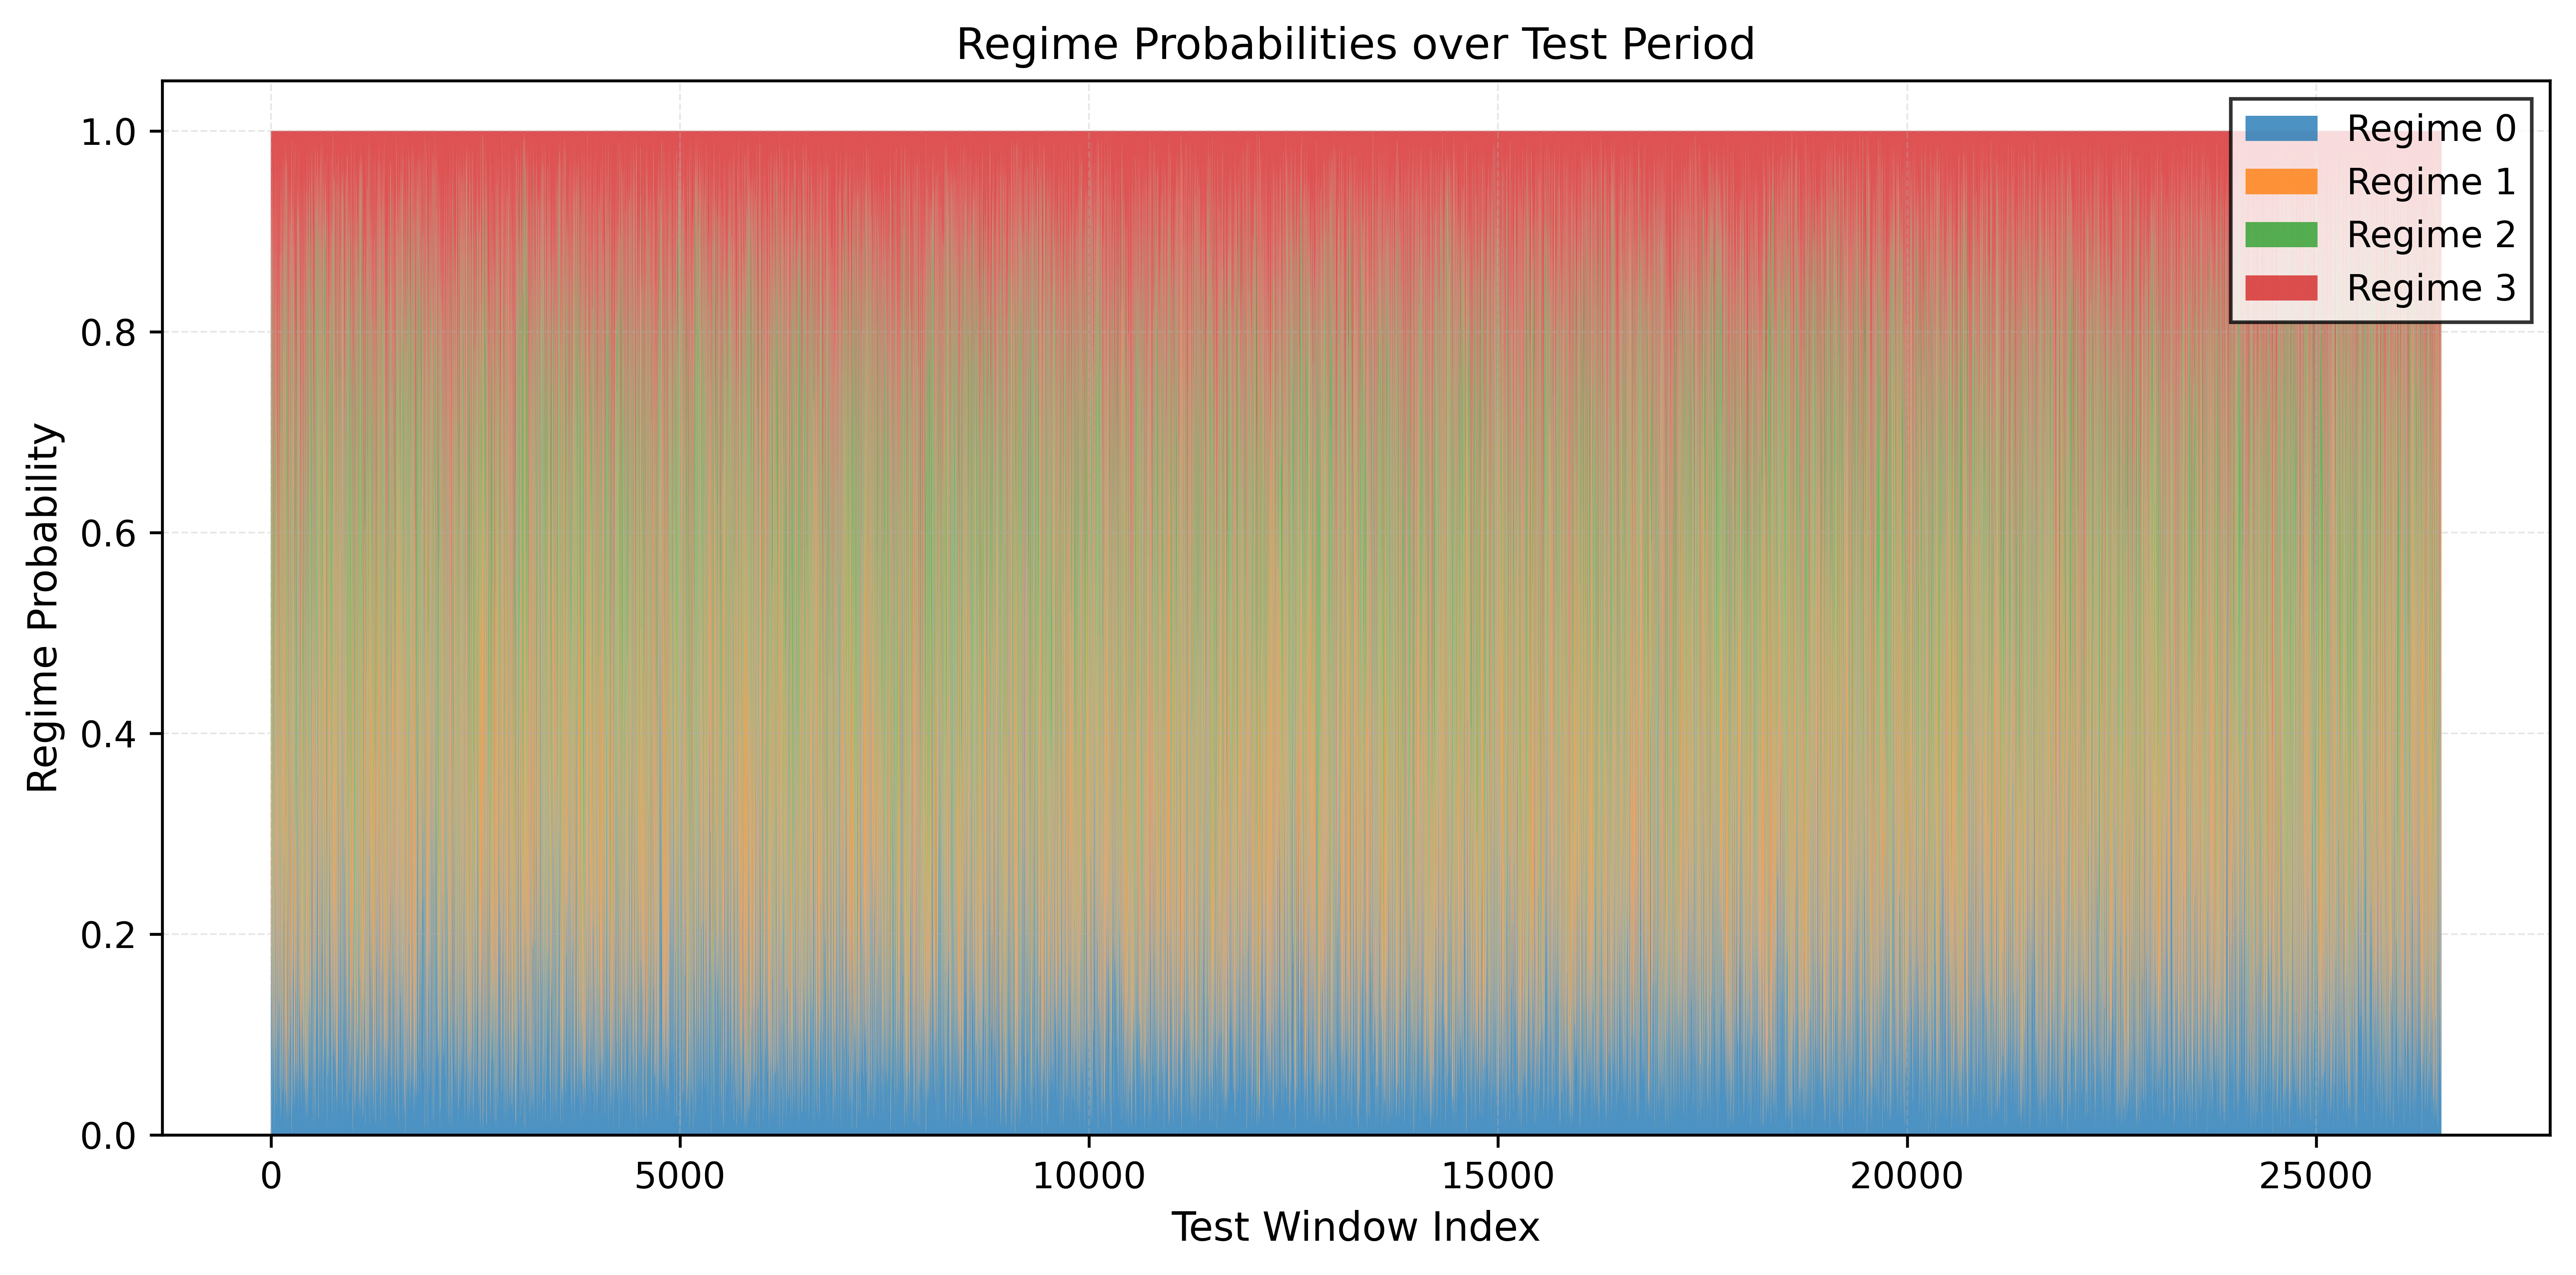
\includegraphics[width=\columnwidth]{plots/regime.png}
    \caption{Model }
    \label{fig:bar}
\end{figure}

HIEU discovers four latent market regimes in an unsupervised manner, exhibiting a balanced distribution across the test period (approximately 24.6-25.7\% per regime). Post-hoc analysis using BTC as a proxy reveals meaningful distinctions: Regime 3 is characterized by the highest average return (+0.0071) and lowest volatility (0.3925), consistent with stable bullish or low-volatility trending phases, while Regime 0 shows pronounced negative returns of minus 0.0115 and elevated volatility (0.4004), likely capturing corrective or bearish conditions. Performance also varies across regimes, with MSE ranging from 0.473 to 0.505, indicating that HIEU adapts predictions to different market dynamics, thereby supporting its regime-aware capability and providing interpretable insights into how temporal shifts and volatility patterns influence forecasting outcomes.


\subsection{Ablation Study}

\begin{table}[h]
\centering
\caption{Ablation study results for HIEU. $\Delta$MSE indicates the relative change in MSE (\%) with respect to the full model.}
\adjustbox{max width=\columnwidth}{%
\begin{tabular}{lrrr}
\toprule
Variant & MSE & MAE & $\Delta$MSE (\%) \\
\midrule
Full HIEU & 0.489 & 0.468 & 0.00 \\
Single Regime & 0.489 & 0.468 & +0.02 \\
No Regime Dimension & 0.489 & 0.468 & +0.02 \\
No Regime Auxiliary Losses & 0.489 & 0.468 & +0.01 \\
No Graph Context & 0.489 & 0.468 & +0.04 \\
No Frequency Reweighting & 0.489 & 0.468 & +0.01 \\
No Hyper Adaptation & 0.489 & 0.468 & +0.01 \\
\bottomrule
\end{tabular}
}
\end{table}






% \begin{table}[h]
% \centering
% \caption{Multi-asset Benchmark Results}
% \begin{tabular}{lrrrrr}
% \toprule
% Model          & MAE      & MSE       & RMSE     & MAPE    & SMAPE   \\
% \midrule
% HIEU           & 0.578   & 1.176    & 1.049   & 125.5   & 170.15  \\
% SimpleMolE     & 0.5793   & 1.1789    & 1.0500   & 122.3   & 171.75  \\
% Linear         & 0.5841   & 1.1929    & 1.0550   & 135.9   & 165.70  \\
% DLinear        & 0.5844   & 1.1934    & 1.0555   & 137.2   & 165.40  \\
% RLinear        & 0.5879   & 1.1959    & 1.0562   & 145.3   & 162.65  \\
% NLLinear       & 0.5888   & 1.1968    & 1.0565   & 148.1   & 162.49  \\
% NLinear        & 0.5891   & 1.1961    & 1.0654   & 148.1   & 162.49  \\
% PatchTST       & 0.5907   & 1.2111    & 1.0620   & 131.2   & 163.94  \\
% \bottomrule
% \end{tabular}
% \end{table}





% \section{Ablation Study}

\section{Conclusion}



%----------------------------------------------------------------------------------------
%	REFERENCES
%----------------------------------------------------------------------------------------
% \begin{thebibliography}{9}
% \clearpage
\bibliographystyle{ACM-Reference-Format}
\bibliography{ijcai26}



% \bibitem[Nie et al.(2023)]{patchtst}
% Nie, Y., Nguyen, N. H., Sinthong, P., \& Kalagnanam, J. (2023).
% \textit{A Time Series is Worth 64 Words: Long-term Forecasting with Transformers.}
% ICLR 2023.

% \bibitem[Liu et al.(2024)]{itransformer}
% Liu, Y., Hu, T., Zhang, H., Wu, H., Wang, S., Ma, L., \& Long, M. (2024).
% \textit{iTransformer: Inverted Transformers are Effective for Time Series Forecasting.}
% ICLR 2024.

% \bibitem[Zeng et al.(2023)]{dlinear}
% Zeng, A., Chen, M., Zhang, L., \& Xu, Q. (2023).
% \textit{Are Transformers Effective for Time Series Forecasting?}
% AAAI 2023.

% \bibitem[Kim et al.(2022)]{revin}
% Kim, T., Kim, J., Tae, Y., Park, C., Choi, J. H., \& Choo, J. (2022).
% \textit{Reversible Instance Normalization for Accurate Time-Series Forecasting against Distribution Shift.}
% ICLR 2022.

% \bibitem[Zhou et al.(2021)]{informer}
% Zhou, H., Zhang, S., Peng, J., Zhang, S., Li, J., Xiong, H., \& Zhang, W. (2021).
% \textit{Informer: Beyond Efficient Transformer for Long Sequence Time-Series Forecasting.}
% AAAI 2021.

% \bibitem[Wu et al.(2021)]{autoformer}
% Wu, H., Xu, J., Wang, J., \& Long, M. (2021).
% \textit{Autoformer: Decomposition Transformers with Auto-Correlation for Long-Term Series Forecasting.}
% NeurIPS 2021.

% \bibitem[Enguehard et al.(2023)]{enguehard2023}
% Enguehard, J. (2023).
% \textit{Neural Perturbations for Time Series Interpretability.}
% (Placeholder Citation).

% \end{thebibliography}

\end{document}